\section{Lezione 16}

Chi compra vuole comprare da fornitori che siano qualificati e che diano una certa garanzia -> \textbf{CMM}.

\textbf{SPICE}: iniziativa per cercare di trovare una valutazione e un'indicazione di miglioramento sulla qualit� dei processi. Intuizione che migliorando i processi si migliorano i prodotti. Il modello \textbf{SPY} dice che posto sotto ogni processo ci dev'essere un meccanismo capace di misurare come sta andando il processo rispetto a obiettivi di qualit� misurabili. Per chiunque parli di qualit� di processo � molto importante il \textbf{CMMI}:

\begin{itemize}

	\item \textbf{Capability}: capacit� di fare le cose, misurazione di quanto un processo � fatto bene e rispetta i suoi obiettivi;
	\item \textbf{Maturity}: misura qual'� la soglia pi� bassa delle capability di processo su tutti i processi che l'azienda attua. Se un'azienda � brava a fare una cosa ma non lo � a fare le altre non � una buona azienda;
	\item \textbf{Model};
	\item \textbf{Integration}: prima questa cosa era applicata al software, ora anche ad altre cose.

\end{itemize}

La sua logica � che ``non possiamo funzionare che a processi'', le organizzazioni devono imparare a funzionare a processi perch� otterranno il massimo risultato. Si dice che un'organizzazione capace di effettuare miglioramenti sui processi � in grado di fare \textbf{governance}, sinonimo di efficacia, efficienza, mantenibilit� e visione. Gestire la qualit� di processi non sta al Project Manager ma ad uno strato pi� importante che sta sopra, ha una visione pi� ampia e possiede una strategia di lungo periodo riferita al miglioramento. Molte aziende hanno \textit{management} ma non hanno \textit{governance} e ad un certo punto si estinguono perch� non hanno la capacit� di adattarsi ai cambiamenti. Il \textbf{CMM} ha il concetto di \textbf{scala}.

\begin{center}
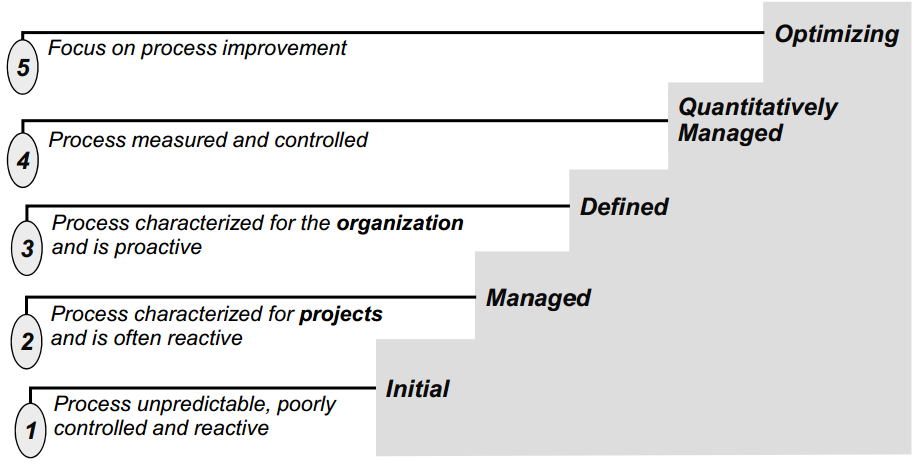
\includegraphics[width=0.75\columnwidth]{img1.png} % Example image
\end{center}

Si parte da osservare che al piano terra c'� uno strato iniziale in cui tutti all'inizio si collocano. I processi, se ci sono, sono a questo stadio \textbf{unpredictable}, impredicibili, \textbf{poorly controlled} e \textbf{reacted}. 

Il livello 2 � \textbf{managed}, cio� gestito. I processi esistono nei progetti e rimangono prevalentemente reattivi. 

Il livello 3 � \textbf{definito}, i processi sono proattivi, esistono trasversalmente, manca ancora il miglioramento. 

Il livello 4 introduce misurazione rispetto al controllo e si chiama \textbf{quantitatively managed}. 

Al livello 5 non soltanto misuriamo ma miglioriamo, \textbf{optimizing}. 

Dove un'azienda si colloca in questa scala dipende fortemente dalla domanda che c'� in un preciso ecosistema (paese). Riflettere su come mi organizzo per effettuare un determinato processo. Adottando il CMMI aumento del 35\% la produttivit�, riduco del 19\% il \textbf{time to market} e riduco del 39\% il \textbf{post-release defect reports} (proporzione di difetti residui, ovvero costi di manutenzione).

\textit{ISO/IEC 15504-2} � un documento simile a CMM che disarticola ogni processo in caratteristiche rilevanti su quel processo e su ogni attributo di processo attacca un'etichetta che dice a che punto siamo su quel processo.

Capito questo bisogna concentrarsi su come lavoriamo, imparare i processi e cercare di migliorarli. Fare lo sforzo di funzionare a processi non � abbastanza, siamo al livello 3, vogliamo almeno andare al 4.